\documentclass[10pt,utf8x]{beamer}

\usepackage{header}

\begin{document}
\setbeamercovered{transparent}

%-------------------------------------------------------------------------------
\begin{frame}
    \makemytitle
\end{frame}
%-------------------------------------------------------------------------------

%-------------------------------------------------------------------------------
\begin{frame}{Concentric wires}
  \begin{columns}[T]
    \column{0.5\linewidth}
    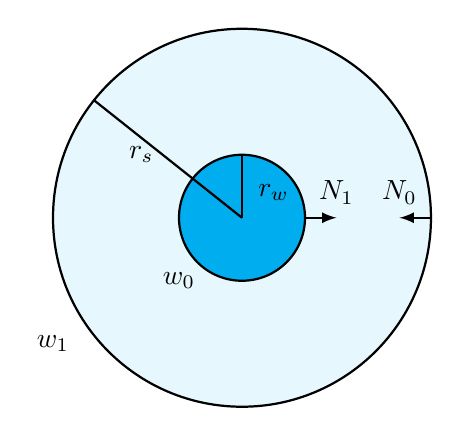
\begin{tikzpicture}[scale=0.8]
      \draw [thick,fill=cyan!10!white]  (0,0) node (v1) {} ellipse (3 and 3);
      \draw [thick,fill=cyan] (0,0) ellipse (1 and 1);
      \draw [thick,-latex] (1,0) -- (1.5,0);
      \draw [thick,-latex](3,0) -- (2.5,0);
      \draw [thick] (0,0) -- (-2.3611,1.8752);
      \draw [thick] (0,0) -- (0,1);
      \node at (-1,-1) {$w_0$};
      \node at (-3,-2) {$w_1$};
      \node at (-1.6,1) {$r_s$};
      \node at (0.5,0.4) {$r_w$};
      \node at (1.5,0.4) {$N_1$};
      \node at (2.5,0.4) {$N_0$};
    \end{tikzpicture}
    \column{0.5\linewidth}
    \begin{itemize}
      \item This example shows a wire $w_1$ include in a shield $w_0$
        and centered in $(0,0)$.
    \end{itemize}
  \end{columns}
\end{frame}
%-------------------------------------------------------------------------------

%-------------------------------------------------------------------------------
\begin{frame}{Multi-wires}
  \begin{columns}[T]
    \column{0.3\linewidth}
    \begin{itemize}
      \item This example shows a shield composed of a wire and a shield which has its own
          wires.
    \end{itemize}
    \column{0.8\linewidth}
    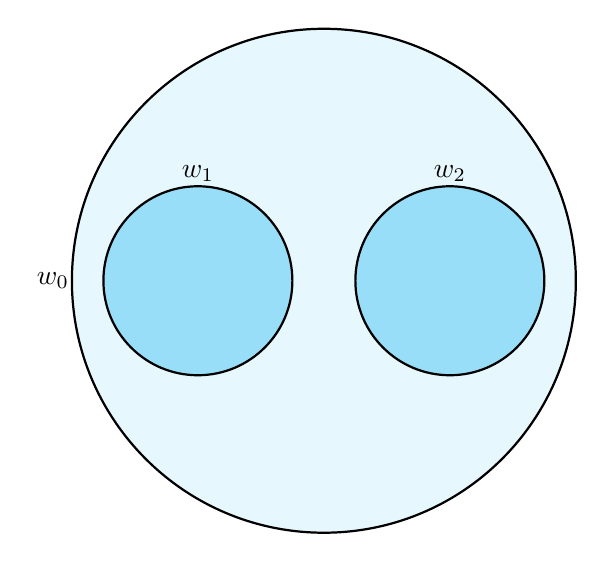
\begin{tikzpicture}[scale=0.8]
      \draw [thick,fill=cyan!10!white]  (0,0) node (v1) {} ellipse (4 and 4);
       \node at (-4.3,0) {$w_0$};
      \draw [thick,fill=cyan!40!white] (-2,0) ellipse (1.5 and 1.5);
       \draw [thick,fill=cyan!40!white] (2,0) ellipse (1.5 and 1.5);
        \node at (-2,1.7) {$w_1$};
        \node at (2,1.7) {$w_2$};

%      \draw [thick,fill=cyan] (2,0) ellipse (0.5 and 0.5);
%      \draw [thick,fill=cyan] (-1.7,0) ellipse (0.5 and 0.5);
%      \draw [thick,fill=cyan] (-0.3,0) ellipse (0.5 and 0.5);
    \end{tikzpicture}
  \end{columns}
\end{frame}
%-------------------------------------------------------------------------------

%-------------------------------------------------------------------------------
\begin{frame}[allowframebreaks]{References}
  \vspace{-0.05\textheight}
  \scriptsize
  \bibliographystyle{apalike}
  \bibliography{seme2014_axessim}
\end{frame}
%-------------------------------------------------------------------------------

%%% Local Variables:
%%% coding: utf-8
%%% mode: latex
%%% TeX-PDF-mode: t
%%% TeX-parse-self: t
%%% TeX-auto-save: t
%%% x-symbol-8bits: nil
%%% TeX-auto-regexp-list: TeX-auto-full-regexp-list
%%% TeX-master: t
%%% ispell-local-dictionary: "american"
%%% End:

\end{document}
